\section{Motivation}

Hydraulic fracturing, commonly known as fracking, is a complex process that involves the initiation and/or propagation of fractures resulting from the application of hydraulic pressure by a fluid. This technique finds extensive applications, particularly in the field of geology. \cite{adachi2007computer}.

In the realm of oil and gas production, fracking is used to stimulate tight shale reservoirs, creating pathways for the extraction of shale gas. Since the pioneering field test at the Hugoton field in 1947, advancements in fracking technology, such as multi-stage hydraulic fracturing and horizontal drilling, have significantly enhanced productivity in these reservoirs. In fact, recent data from the US Energy Information Administration\cite{eia_data_on_gas, eia_data_on_oil} reveals that a significant portion, around 66\% of all oil and 80\% of all gas, produced in the United States comes from wells that undergo hydraulic fracturing. (See Figure \ref{oil_and_gas_production}.)

\begin{figure}[h]
    % \centering
    \begin{subfigure}{.49\textwidth}
      \centering
      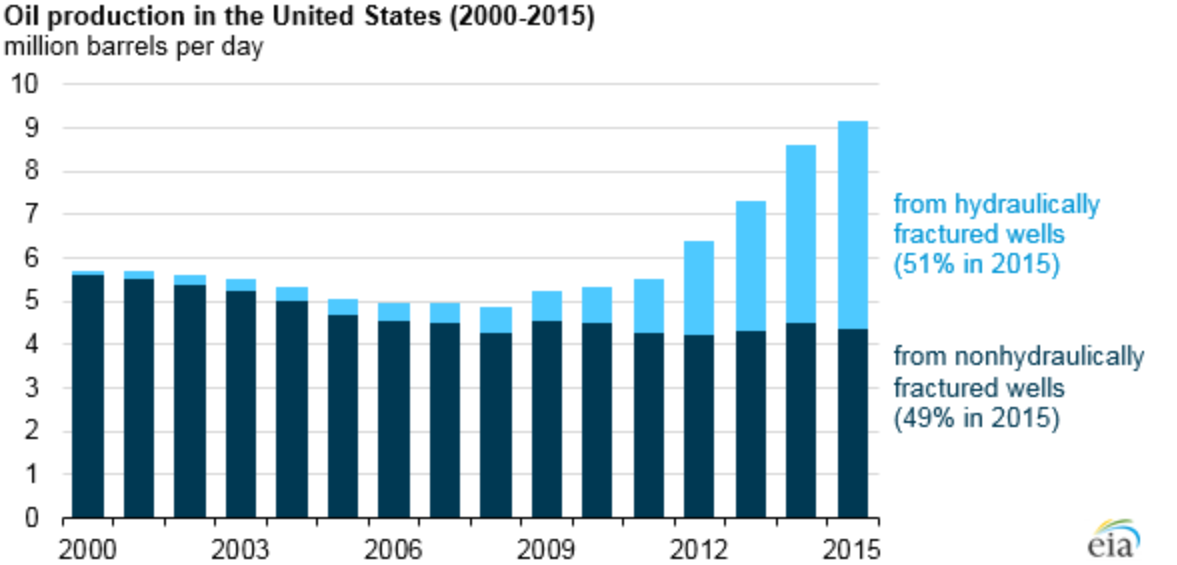
\includegraphics[width=\linewidth]{Chapter1/oil_from_fracs.png}
      \label{fig:oil_fracs}
    \end{subfigure}%
    \begin{subfigure}{.49\textwidth}
      \centering
      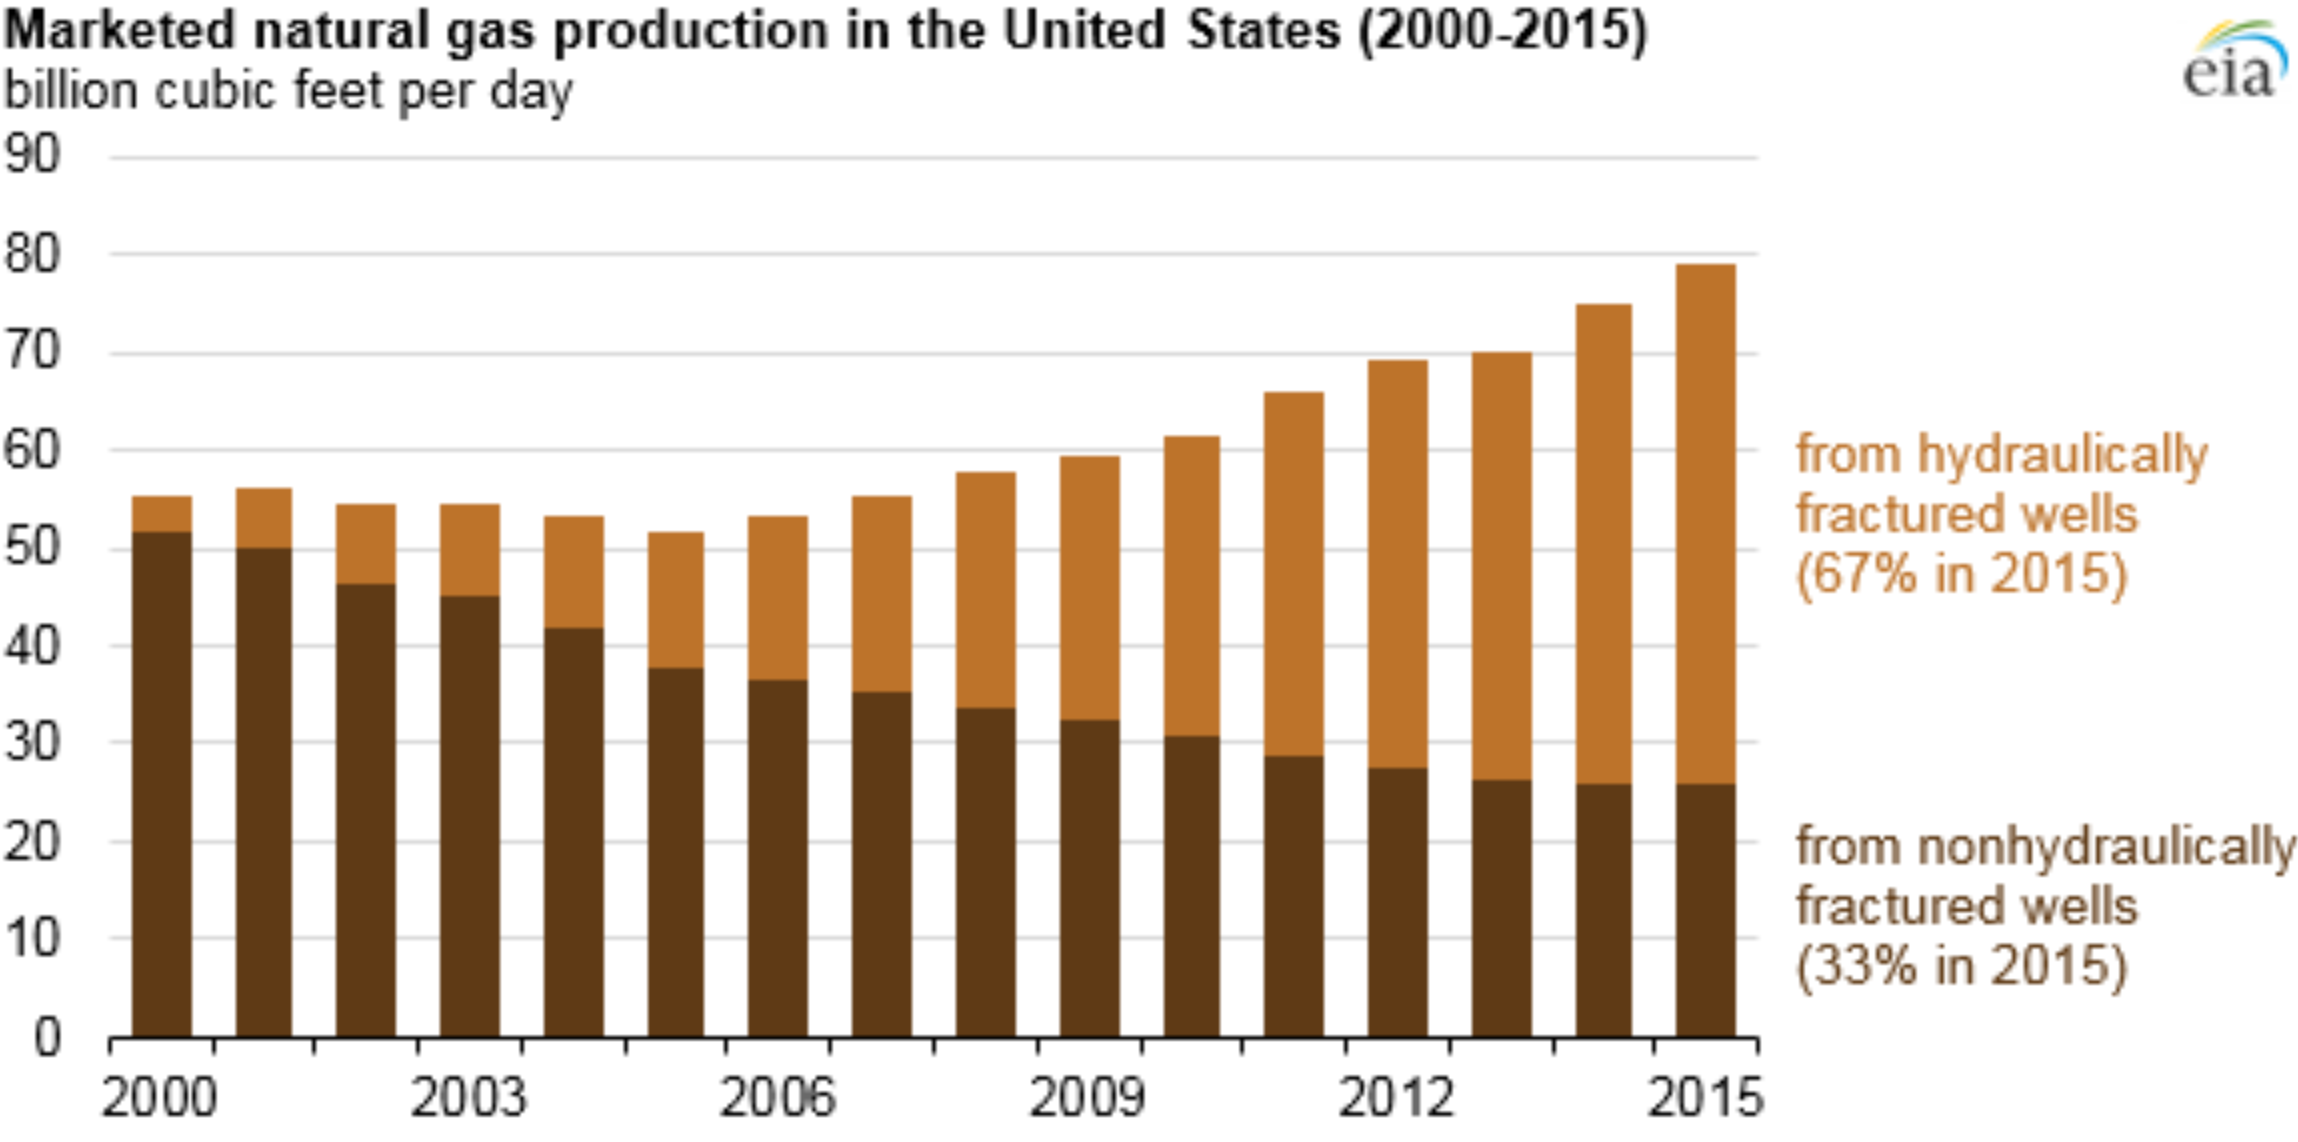
\includegraphics[width=\linewidth]{Chapter1/gas_from_fracs.png}
      \label{fig:gas_fracs}
    \end{subfigure}%
      \caption{These plots show the evolution of fracking, leading to it becoming the main source of oil and gas in the United States. The numbers shown in the graphs are behind the actual values mentioned in the text because the charts were last updated in 2015. Courtesy from the US Energy Information Administration.}
\end{figure}\label{oil_and_gas_production}

Hydraulic fracturing also plays a crucial role in geothermal energy, which offers a promising avenue for generating renewable, carbon-free electricity. In general, the biggest challenge of these geothermal systems is the low permeability of most suitable hot rock formations, which limits the productivity of these systems in their natural state. By employing hydraulic fracturing techniques, the permeability, and consequently the efficiency of geothermal systems can be improved. These specially treated systems are commonly referred to as Enhanced Geothermal Systems (EGS). Advances in fracking science and technology are thus one of the key steps towards making EGS a viable and reliable clean energy source. The process is depicted in Figure \ref{egs-wrap}.

\begin{wrapfigure}{R}{5cm}
    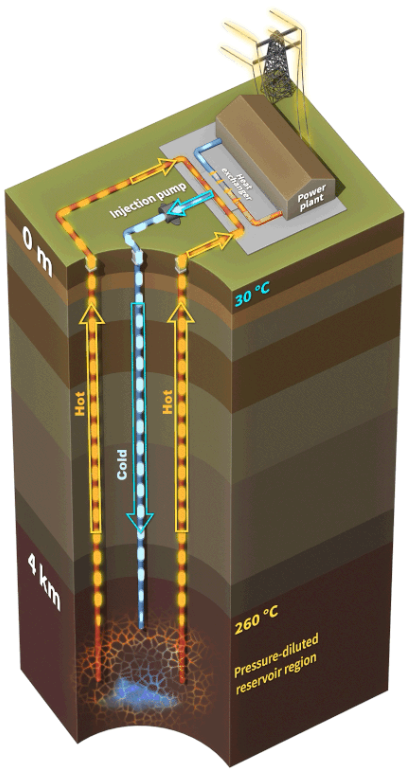
\includegraphics[width=5.5cm]{Chapter1/geothermal.png}
    \caption{Simplied depiction of an EGS system. Courtesy of Los Alamos National Laboratory.}\label{egs-wrap}
\end{wrapfigure} 

Another significant geological process that addresses the global CO2 problem is Carbon Storage and Sequestration, where CO2 is injected and trapped in tight rock formations deep beneath the surface, preventing its release into the atmosphere. In the context of CO2 sequestration, caprock fracturing, which can happen during injection or through long-term thermo-chemo-mechanical processes may lead to CO2 leakage.\cite{pan2014tough} This consists thus of case where, in contrast of the previous ones, hydraulic fracture must be prevented. 

One can also find applications in various other fields, including the disposal of waste drill cuttings underground \cite{moschovidis_mounds_2000}, measurement of in situ stresses \cite{desroches_stress_1995, desroches1993modelling}, goafing and fault reactivation in mining operations \cite{board_fluid_1992, zhang_propagation_2002}, and stimulation of groundwater wells \cite{noauthor_permeability_nodate,less_hydrofracture_1994}.

Despite its significant economic benefits, the process has raised concerns among critics regarding potential seismic events, especially in the context of O\&G and EGS applications. Additional objections center around the environmental impact, including air and noise pollution, as well as the risk of groundwater and surface water contamination when chemicals are mixed with the injection fluids.

Given the importance of these applications and the associated risks, it is evident that a comprehensive understanding of fracture processes is crucial for the well-being of our planet and society. However, obtaining sufficient experimental data for deep subsurface processes is challenging due to the depths involved and the difficulty in replicating true rock conditions in laboratory experiments. Consequently, there has been a growing focus on computational modeling and simulation of fluid-driven fracture. These computational approaches provide a cost-effective means to gain insights into the intricate physical processes associated with hydraulic fracturing.

